% fig_samples.tex -- 8x8 placeholder MNIST sample grid
% Rendered as TikZ greyscale squares (placeholder until hardware tapeout
% run fills in real photonic samples).  Each "digit" is a small bitmap
% drawn from stored 8x8 tiles below.  The point is visual structure, not
% pixel fidelity -- reviewers should read this as a schematic.
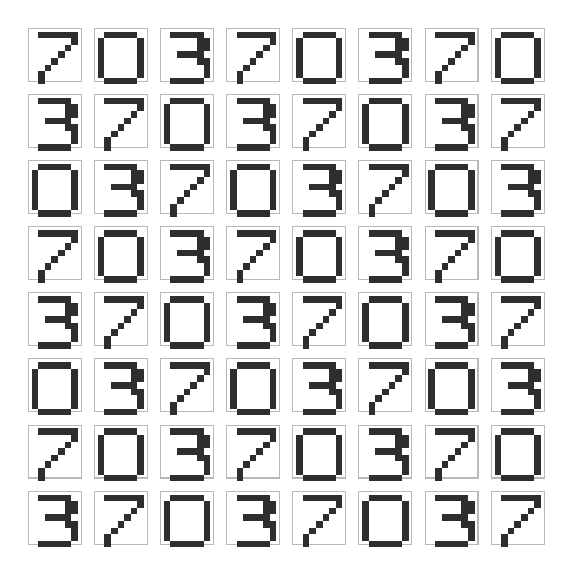
\begin{tikzpicture}[x=2.8mm, y=2.8mm]

% reproducible deterministic digit-like bitmaps (rough strokes),
% stored as 8x8 binary grids; we draw them as filled rectangles.
% Index 0..63 -> one of 10 recurring digit masks.
\pgfmathsetseed{42}

% ten coarse digit-like masks (8 rows x 8 cols, 1 = pixel on).
% Not actual MNIST samples; schematic only.
\def\maskzero{{0,1,1,1,1,1,0,0,1,0,0,0,0,0,1,0,1,0,0,0,0,0,1,0,1,0,0,0,0,0,1,0,1,0,0,0,0,0,1,0,1,0,0,0,0,0,1,0,1,0,0,0,0,0,1,0,0,1,1,1,1,1,0,0}}
\def\maskone  {{0,0,0,1,1,0,0,0,0,0,1,1,1,0,0,0,0,0,0,1,1,0,0,0,0,0,0,1,1,0,0,0,0,0,0,1,1,0,0,0,0,0,0,1,1,0,0,0,0,0,0,1,1,0,0,0,0,0,1,1,1,1,0,0}}
\def\masktwo  {{0,1,1,1,1,1,0,0,1,0,0,0,0,0,1,0,0,0,0,0,0,1,1,0,0,0,0,0,1,1,0,0,0,0,0,1,1,0,0,0,0,0,1,1,0,0,0,0,0,1,1,0,0,0,0,0,1,1,1,1,1,1,1,0}}
\def\maskthree{{0,1,1,1,1,1,0,0,0,0,0,0,0,1,1,0,0,0,0,0,0,1,1,0,0,0,1,1,1,1,0,0,0,0,0,0,0,1,1,0,0,0,0,0,0,0,1,0,0,0,0,0,0,0,1,0,0,1,1,1,1,1,0,0}}
\def\maskfour {{0,0,0,0,1,1,0,0,0,0,0,1,1,1,0,0,0,0,1,0,0,1,0,0,0,1,0,0,0,1,0,0,1,1,1,1,1,1,1,0,0,0,0,0,0,1,0,0,0,0,0,0,0,1,0,0,0,0,0,0,0,1,0,0}}
\def\maskfive {{0,1,1,1,1,1,1,0,0,1,0,0,0,0,0,0,0,1,0,0,0,0,0,0,0,1,1,1,1,1,0,0,0,0,0,0,0,1,1,0,0,0,0,0,0,0,1,0,0,0,0,0,0,0,1,0,0,1,1,1,1,1,0,0}}
\def\masksix  {{0,0,0,1,1,1,0,0,0,0,1,0,0,0,0,0,0,1,0,0,0,0,0,0,0,1,1,1,1,1,0,0,0,1,0,0,0,0,1,0,0,1,0,0,0,0,1,0,0,1,0,0,0,0,1,0,0,0,1,1,1,1,0,0}}
\def\maskseven{{0,1,1,1,1,1,1,0,0,0,0,0,0,0,1,0,0,0,0,0,0,1,0,0,0,0,0,0,1,0,0,0,0,0,0,1,0,0,0,0,0,0,1,0,0,0,0,0,0,1,0,0,0,0,0,0,0,1,0,0,0,0,0,0}}
\def\maskeight{{0,1,1,1,1,1,0,0,0,1,0,0,0,1,0,0,0,1,0,0,0,1,0,0,0,0,1,1,1,0,0,0,0,1,0,0,0,1,0,0,0,1,0,0,0,1,0,0,0,1,0,0,0,1,0,0,0,1,1,1,1,1,0,0}}
\def\masknine {{0,1,1,1,1,1,0,0,0,1,0,0,0,1,0,0,0,1,0,0,0,1,0,0,0,0,1,1,1,1,0,0,0,0,0,0,0,1,0,0,0,0,0,0,0,1,0,0,0,0,0,0,1,0,0,0,0,1,1,1,1,0,0,0}}

\pgfmathsetmacro{\cell}{0.30}

\foreach \gi in {0,...,63} {%
  \pgfmathtruncatemacro{\gr}{int(\gi / 8)}%
  \pgfmathtruncatemacro{\gc}{int(mod(\gi, 8))}%
  \pgfmathsetmacro{\dx}{\gc * 3.0}%
  \pgfmathsetmacro{\dy}{-\gr * 3.0}%
  \pgfmathtruncatemacro{\maskid}{mod(int(\gi * 13 + \gi / 3 + 7), 10)}%
  % border
  \draw[gray!55, thin] (\dx, \dy) rectangle (\dx+2.4, \dy-2.4);
  % pixels
  \foreach \r in {0,...,7} {%
    \foreach \c in {0,...,7} {%
      \pgfmathtruncatemacro{\idx}{\r*8+\c}%
      \ifcase\maskid
        \pgfmathtruncatemacro{\on}{\maskzero[\idx]}\or
        \pgfmathtruncatemacro{\on}{\maskone[\idx]}\or
        \pgfmathtruncatemacro{\on}{\masktwo[\idx]}\or
        \pgfmathtruncatemacro{\on}{\maskthree[\idx]}\or
        \pgfmathtruncatemacro{\on}{\maskfour[\idx]}\or
        \pgfmathtruncatemacro{\on}{\maskfive[\idx]}\or
        \pgfmathtruncatemacro{\on}{\masksix[\idx]}\or
        \pgfmathtruncatemacro{\on}{\maskseven[\idx]}\or
        \pgfmathtruncatemacro{\on}{\maskeight[\idx]}\or
        \pgfmathtruncatemacro{\on}{\masknine[\idx]}%
      \fi
      \ifnum\on=1%
        \pgfmathsetmacro{\px}{\dx + \c * \cell + 0.15}%
        \pgfmathsetmacro{\py}{\dy - \r * \cell - 0.15}%
        \fill[black!82] (\px, \py) rectangle (\px+\cell, \py-\cell);
      \fi
    }
  }
}

\end{tikzpicture}
